\section{Current results}

Problem:
A car with fully-observable 2D-state: [position, velocity] needs to move from initial position $x_0=0$\si{\metre} and initial velocity $v_0=0$\si{\metre\per\ts} to goal position $x_F=\SI{2.0}{\metre}$. At every time-step \si{\ts}, with a discretization of $t_d=0.1$, the car receives an acceleration as a control input. The control input $a$ is constrained to range between [-1.0,1.0]\si{\metre\per\square\ts}.
Per every time-step passed before it reaches the goal, it receives a penalization reward $R_{\tau}=-1$ 
If the car reaches the goal position, it receives a reward $R_F=100$ and the episode ends. Otherwise, after $T_F=400$\si{\ts} the episode ends (with no extra penalization).

\subsection{Case 1: No velocity penalization}
Both DDPG and CVAR-DDPG manage to arrive with linear increment in velocity with a slope of 2.
(Accelearation at maximum during the whole episode).
For this setup we have:

\begin{equation*}
    x = x_0 + v_0 \frac{\si\ts}{10} + 0.5a \big ( \frac{\si\ts}{10} \big )^2
\end{equation*}
In the optimal case, the car keeps an acceleration of 1\si{\metre\per\square\ts} for the whole episode, and hence reaches $x_F=2$\si{\metre} with 20 time-steps.
Hence the final cumulative reward $G_T= (20+1) R_{\tau} + R_{F}=70$.
\textbf{add pics}
\todo{add pics}

\subsection{Case 2: Velocity penalization with probability 1 }
The experiment is carried out to ensure the two algorithms manage to learn the new reward function when there is no uncertainty. \\

In this setup, when the car velocity exceeds 1\si{\metre\per\ts}, it receives a penalization of $R_v=-20$.
We expect both algorithms to perform similarly since there is no reward uncertainty.\\
As expected, both algorithms learn to accelerate with maximum value till a velocity of 1\si{\metre\per\ts} is reached, and then keeping this velocity constant until the goal is reached.\\

Starting from $x_0=0$\si\metre, the car reaches a velocity of 1\si{\metre\per\ts} after 10 time-steps, at $x_{\tau=10}=0.5$. Keeping velocity 1\si{\metre\per\ts} through the rest of the episode,
it reaches the goal position after $14$ time-steps. Hence the final cumulative reward $G_T= (10+14+1) R_{\tau} + R_{F}=74$.
The reward values were chosen in order to make sure that, for this Case 2 setting, driving with a velocity higher than 1\si{\metre\per\ts} never induces higher cumulative rewards.\\

\textbf{For this Case 2 setting, the trained models were saved using Early stopping with \textit{maximal reward in episode evaluation} as a metric and with a patience of 100 episodes.}\\
The quantiles used for learning the actor for the CVAR-DDPG algorithm were sampled uniformly $\backsim\ U[0,1] $

\begin{figure}[ht]
        \centering
        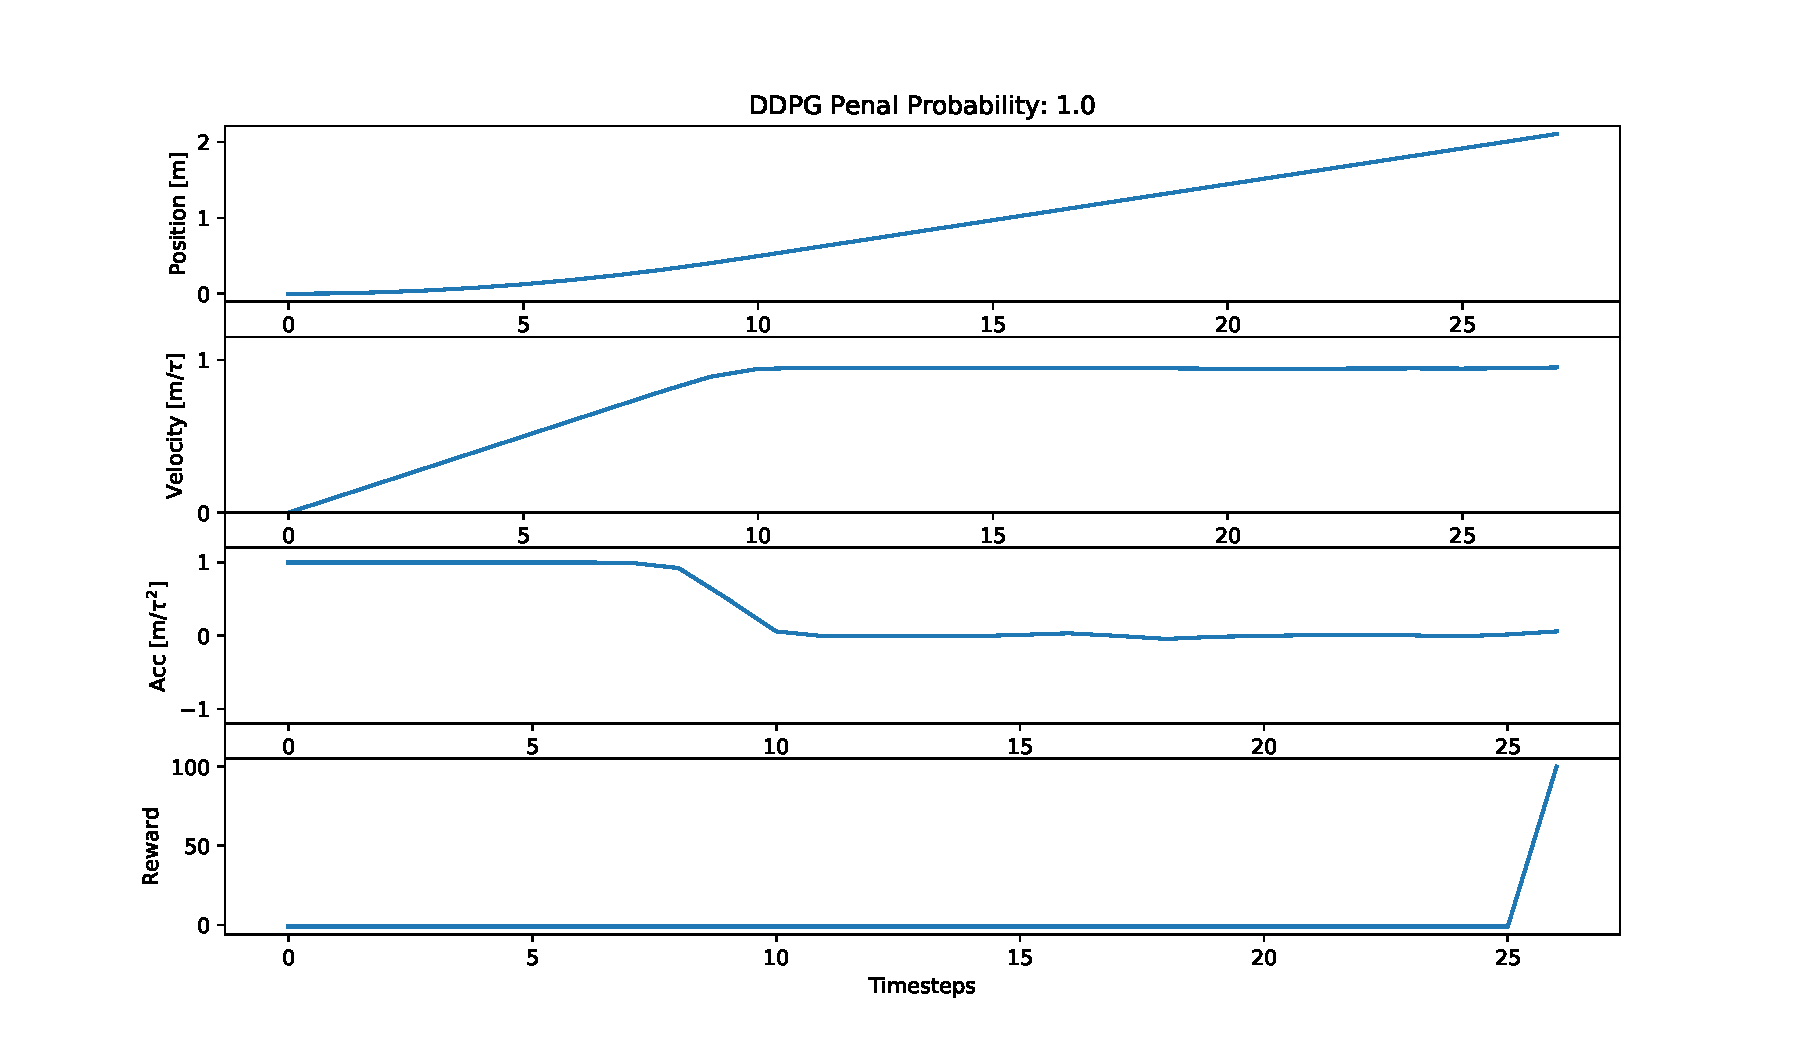
\includegraphics[width=0.8\textwidth]{images/DDPG/Trajectory_DDPG_ppenal1.pdf}
        \caption{Car trajectory using DDPG algorithm and velocity penalization with probability 1 }
        \label{traj1_ddpg_probpenal1}
    
\end{figure}


\begin{figure}[ht]
        \centering
        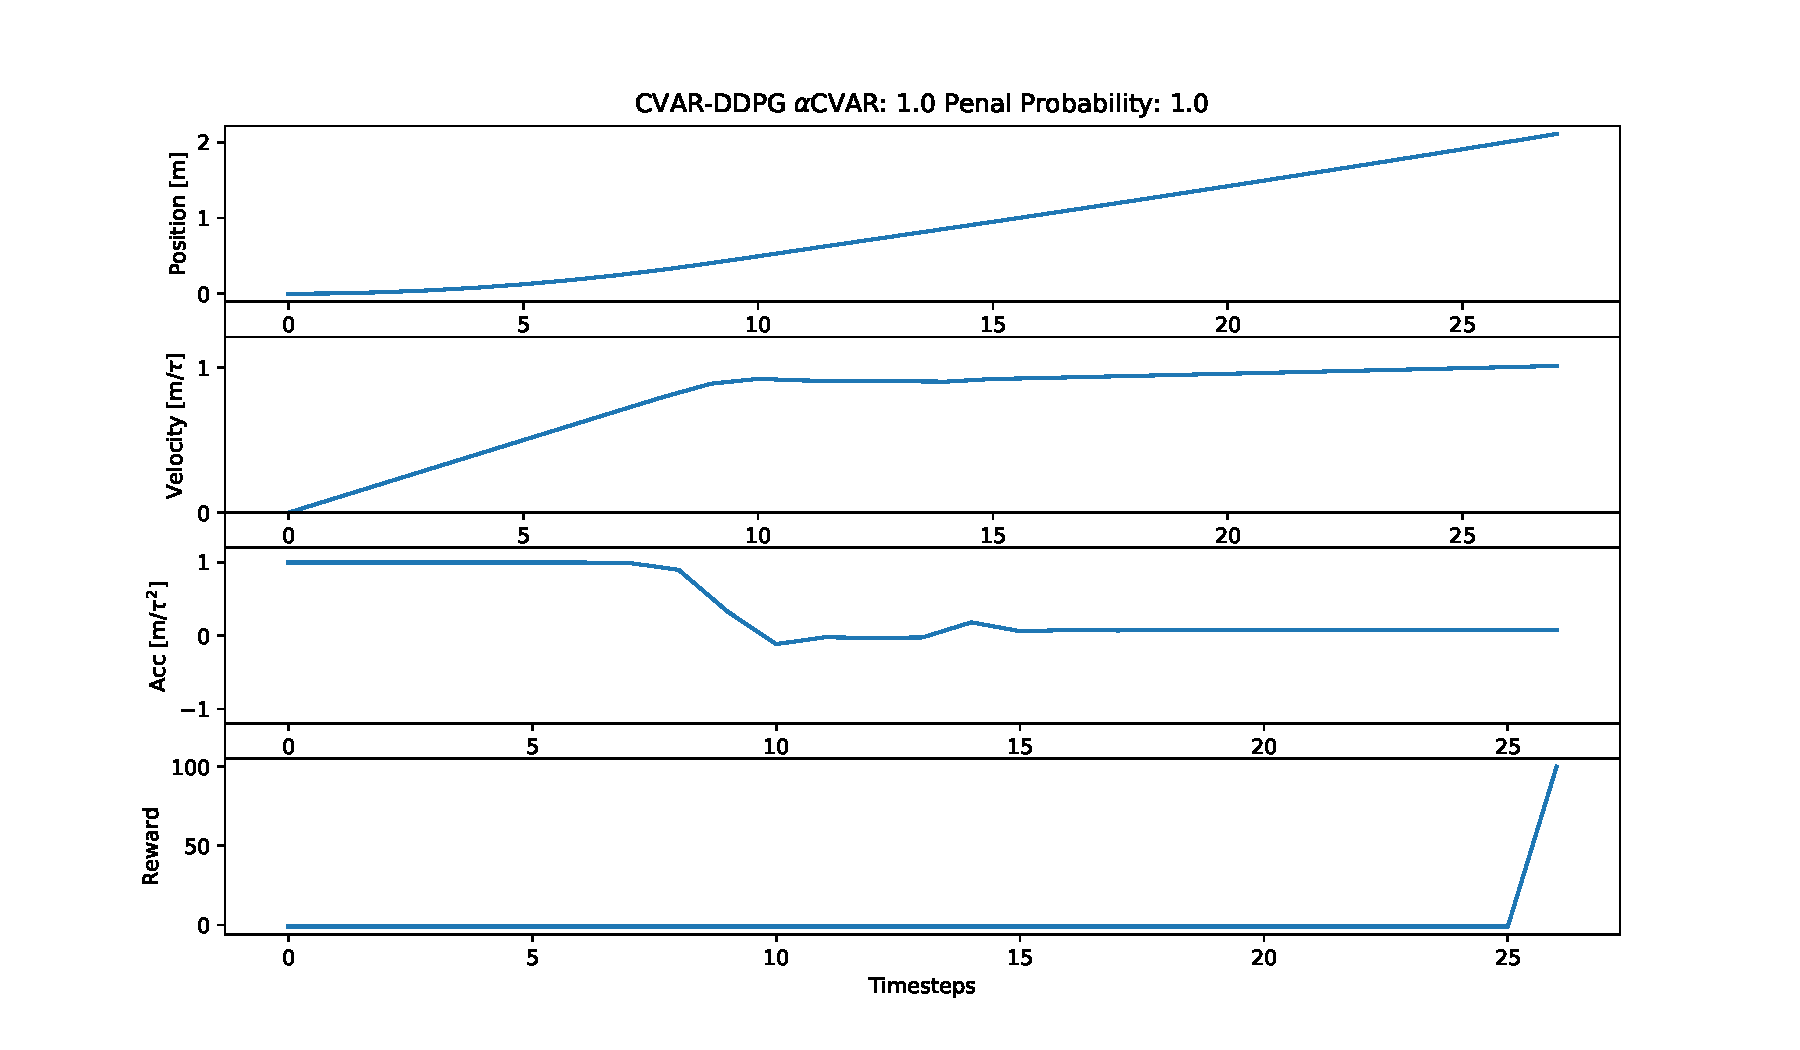
\includegraphics[width=0.8\textwidth]{images/CVAR/Trajectory_CVAR_ppenal1.pdf}
        \caption{Car trajectory using CVAR-DDPG algorithm and velocity penalization with probability 1. ($\alpha$-CVAR = 1)}
        \label{traj_cvarddpg_probpenal1_cvar1}
    
\end{figure}

\newpage
\subsection{Case 3: Velocity penalization with probability P }
The experiment is carried out to show the risk-sensitiveness property of the CVAR-DDPG algorithm.\\

\textbf{The models saved were the ones that obtained a maximum CVAR (with a window of 10 episodes)
of the cumulative rewards during evaluation}\\
The quantiles used for learning the actor for the CVAR-DDPG algorithm were sampled uniformly $\backsim\ U[0,\alpha] $ where $\alpha=0.2$\\

For P=0.2 the CVAR-DDPG algorithm learns to saturate the velocity, even though the probability of a penalization is low, whereas the DDPG algorithm doesn't, and keeps a linear increase of the velocity during the whole episode.
The CVAR algorithm reaches its maximum CVAR of 64.0 at episode 220, whereas the DDPG reaches its maximum CVAR value of 49.0 at episode 1435.\\

\textbf{Important issue}: Although CVAR-DDPG finds a risk-sensitive trajectory at episode 220, it doesn't converge there and keeps oscillating and even moves towards a risk-neutral behaviour later on.\\
The graph in figure \ref{tail_CDF_EVOL} , shows the evolution of the sampled mean of the tail of the sampled cumulative value distribution (CDF). (ie we compute via IQN the quantile values from the tail value distribution (VD) and take the mean).
The value it converges to coincides with the maximum value of the CVAR we achieved ,but then the actor doesn't seem to behave accordingly.\\


\begin{equation}
        \text{CVaR}_\alpha (Z) = \frac{1}{\alpha} \int_{0}^{\alpha} F^{-1}_Z(\tau) d\tau=\frac{1}{\alpha} \int_{0}^{\alpha} IQN(\tau) d\tau \approx 
        \frac{1}{\alpha} \frac{1}{K}\sum_{i=0}^K IQN(\tau_i) 
\end{equation}
where $\tau_i \sim U[0,\alpha]$, and IQN is the output of the IQN network for given $\tau$, representing the
value of the return for the given quantile.\\
(Values of the sampled CVAR showed in \ref{tail_CDF_EVOL} are not divided by $\alpha$ neither K )
\begin{figure}[ht]
        \centering
        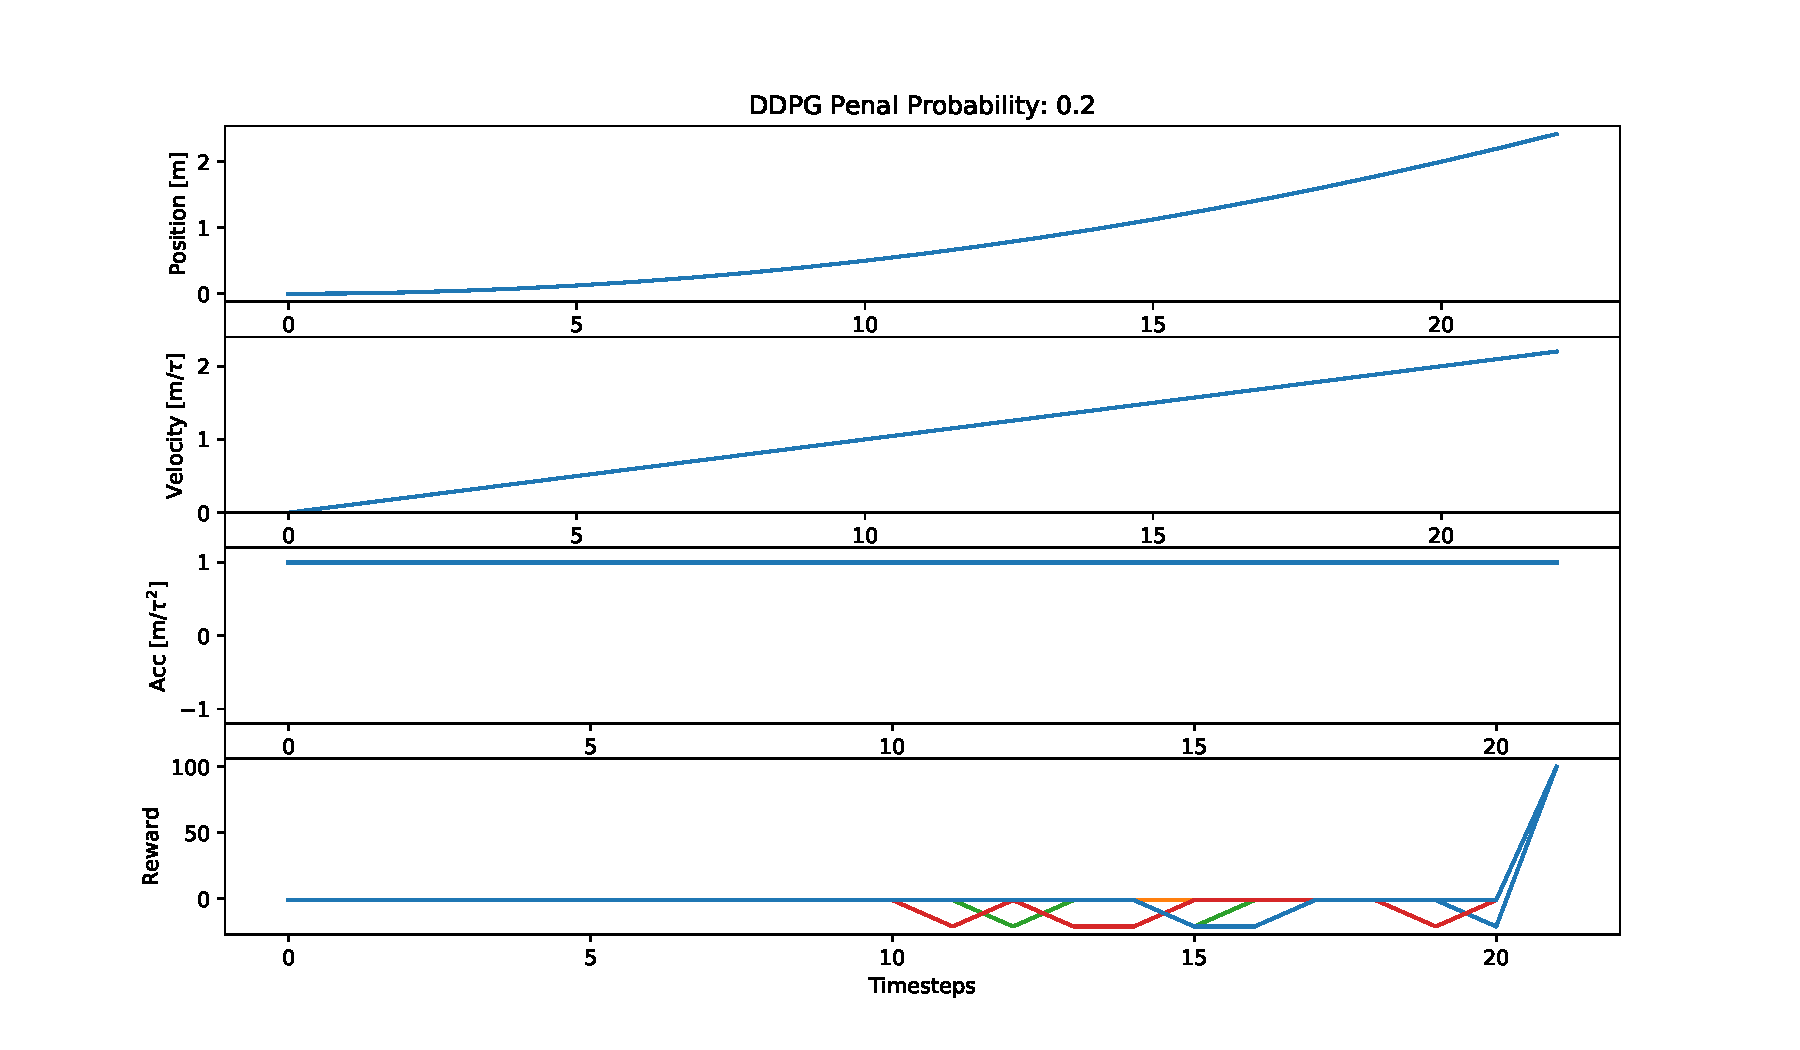
\includegraphics[width=0.8\textwidth]{images/DDPG/Trajectory_DDPG_ppenal02.pdf}
        \caption{Car trajectory using DDPG algorithm and velocity penalization with
        probability P=0.2}
        \label{traj_ddpg_probpenal0.2}
    
\end{figure}
\begin{figure}[ht]
        \centering
        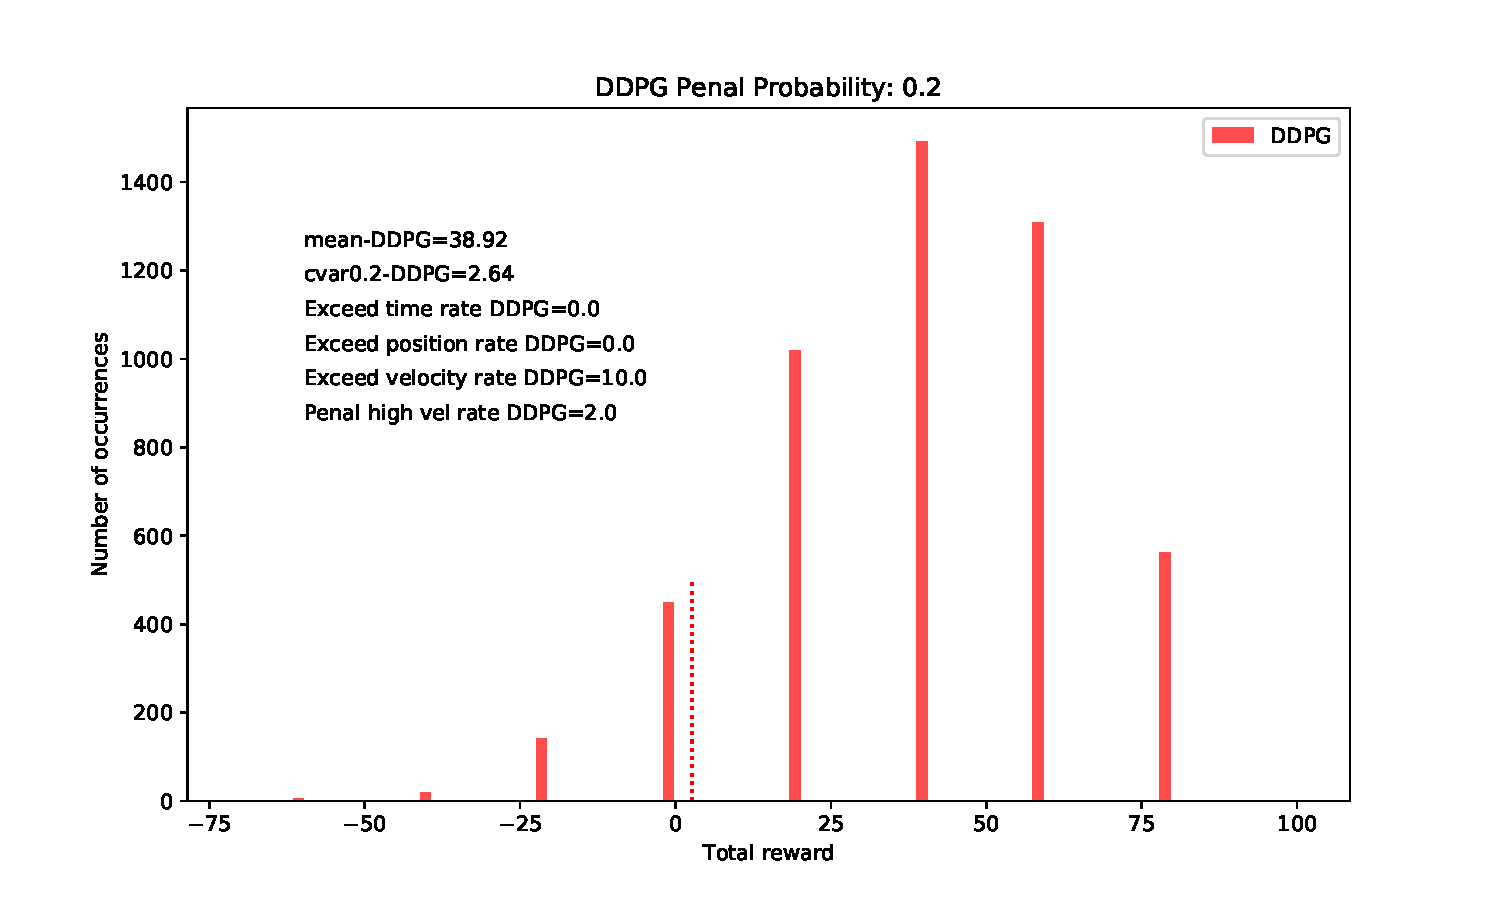
\includegraphics[width=0.8\textwidth]{images/DDPG/Rewards_DDPG_ppenal02.pdf}
        \caption{Reward distribution using DDPG algorithm and velocity penalization with probability 0.2}
        \label{rew_ddpg_probpenal0.2}
    
\end{figure}


\begin{figure}[ht]
        \centering
        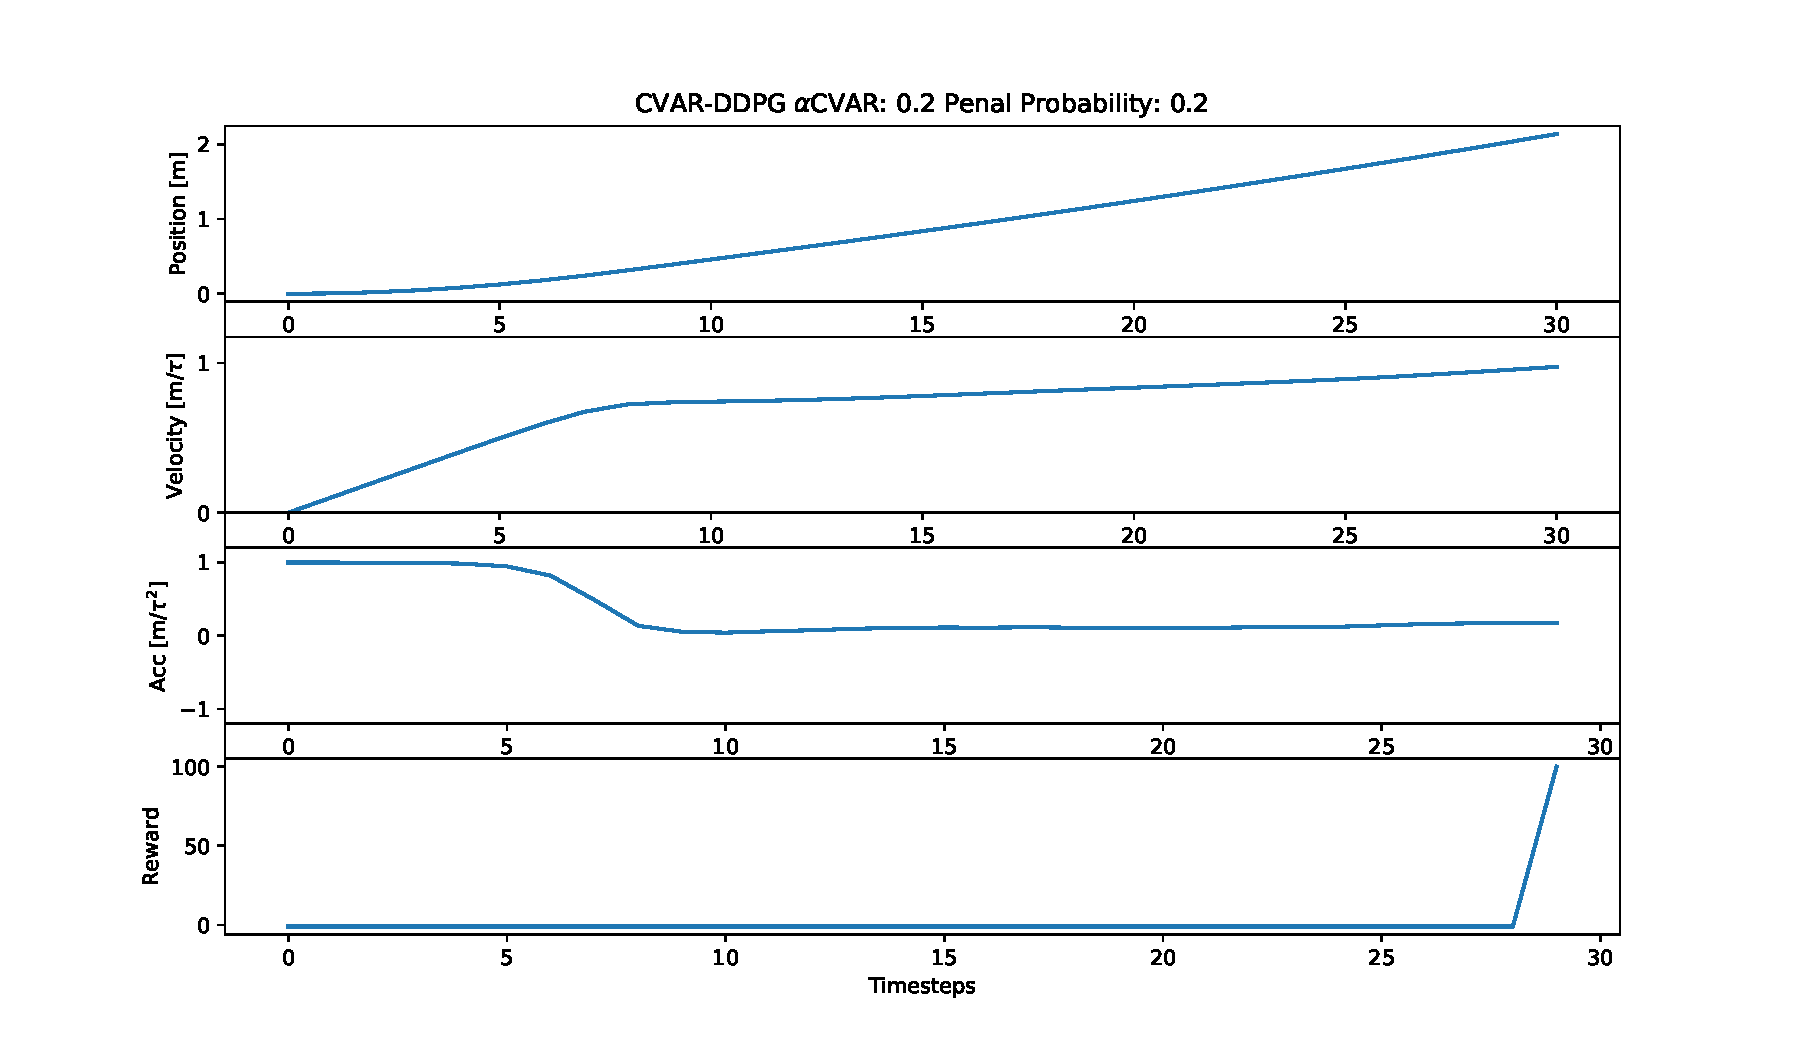
\includegraphics[width=0.8\textwidth]{images/CVAR/Trajectory_CVAR_ppenal02.pdf}
        \caption{Car trajectory using CVAR-DDPG algorithm and velocity penalization with probability 0.2 and ($\alpha$-CVAR = 0.2)}
        \label{traj_cvar_ddpg_probpenal0.2_cvar0.2}
    
\end{figure}

\begin{figure}[ht]
        \centering
        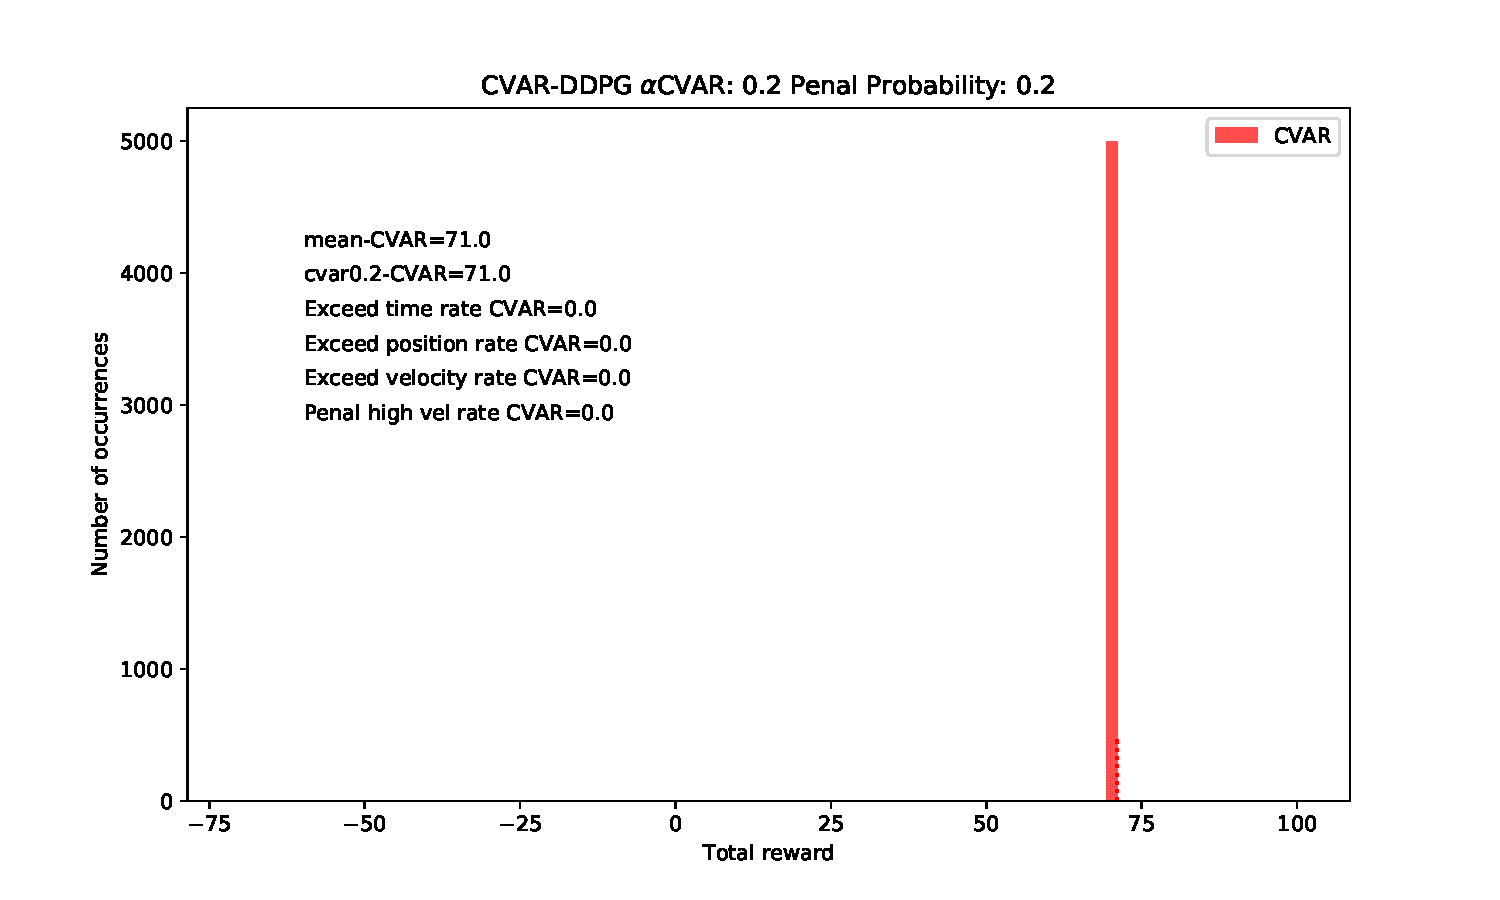
\includegraphics[width=0.8\textwidth]{images/CVAR/Rewards_CVAR_ppenal02.pdf}
        \caption{Reward distribution using CVAR-DDPG algorithm and velocity penalization with probability 0.2 and ($\alpha$-CVAR = 0.2)}
        \label{rew_cvar_ddpg_probpenal0.2_cvar0.2}
    
\end{figure}
\begin{figure}[ht]
        \centering
        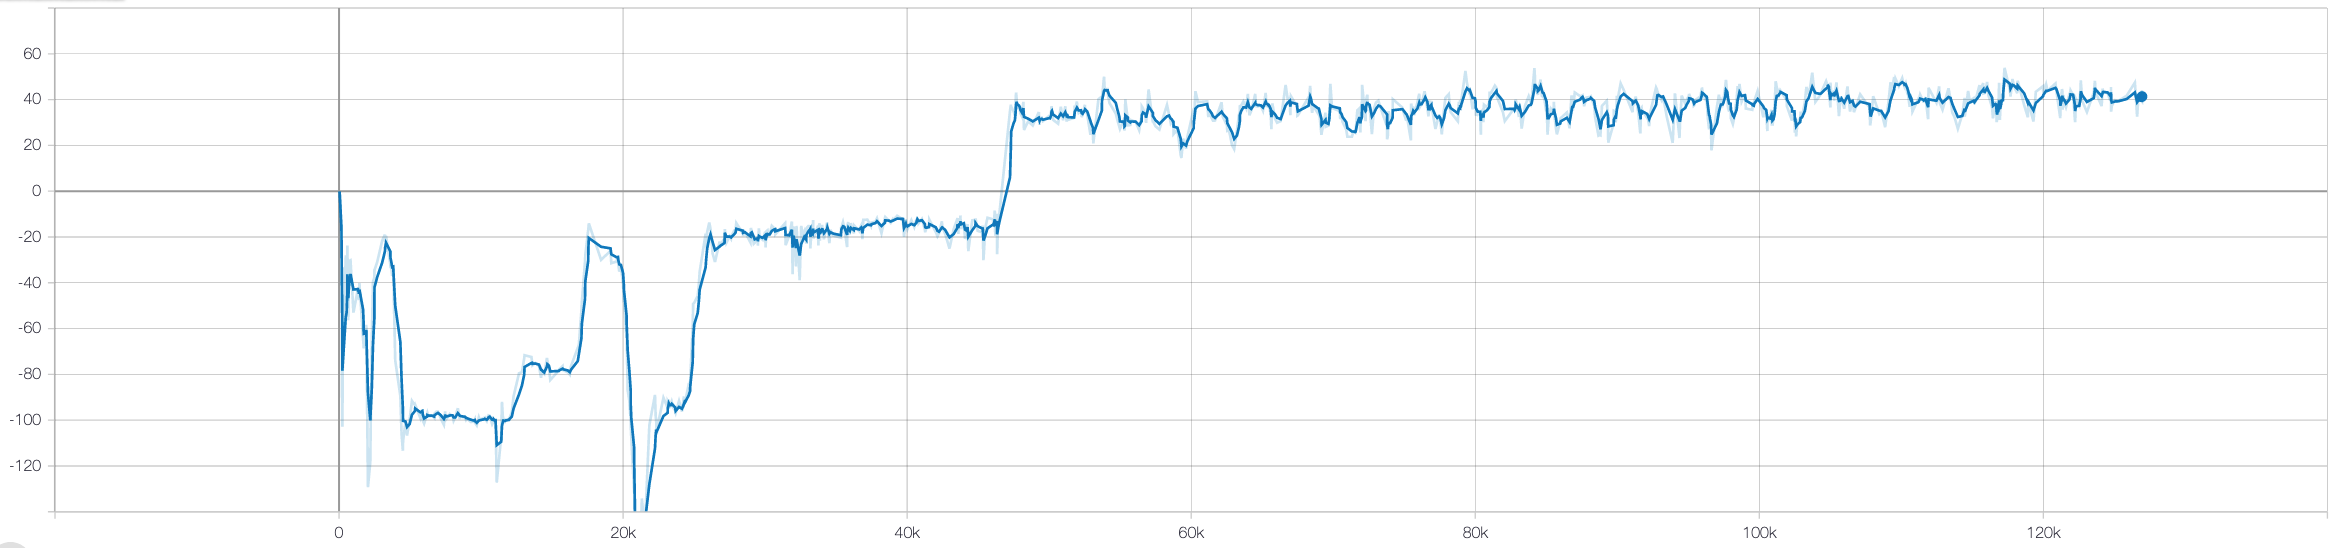
\includegraphics[width=0.8\textwidth]{images/CVAR/Cvar_evol.png}
        \caption{Evolution of the sampled mean of the tail of the Cumulative Value Distribution during training epochs}
        \label{tail_CDF_EVOL}
    
\end{figure}




\end{document}


\section{Old}
Considering that the common DDPG failure of the critic overestimation problem could be the issue, we moved from CVAR-DDPG algorithm to CVAR-TD3 algorithm.
No success. Still learning really slow trajectories till the actor-loss blows down.


\begin{figure}[t]
        \centering
        \includegraphics[width=0.8\textwidth]{images/Rewards_CVAR_TD3_penal_prob0.3_cvar0.1.png}
        \caption{Reward distribution using CVAR-TD3 algorithm and velocity penalization with probability 0.3 and ($\alpha$-CVAR = 0.1)}
        \label{rew_cvar_td3_probpenal0.3_cvar0.1}
    
\end{figure}

\begin{figure}[t]
        \centering
        \includegraphics[width=0.8\textwidth]{images/Traj_CVAR_TD3_penal_prob0.3_cvar0.1.png}
        \caption{Car trajectory using CVAR-TD3 algorithm and velocity penalization with probability 0.3 and ($\alpha$-CVAR = 0.1)}
        \label{traj_cvar_td3_probpenal0.3_cvar0.1}
    
\end{figure}

\begin{figure}[t]
    \begin{minipage}[t]{.5\textwidth}
        \centering
        \includegraphics[width=0.8\textwidth]{images/Actor_loss_DDPG_algorithms.png}
        \caption{Actor loss DDPG algorithm with velocity penalization with prob 0.3.}
        \label{ddpg_actor_loss}
    \end{minipage}%
    \hfill%
    \begin{minipage}[t]{.5\textwidth}
        \centering
        \includegraphics[width=\textwidth]{images/Actor_loss_CVAR_algorithms.png}
        \caption{Actor loss of several CVAR algorithms showing blowing up of losses.}
        \label{cvar_actor_loss}
    \end{minipage}
\end{figure}


\begin{figure}[t]
        \centering
        \includegraphics[width=0.8\textwidth]{images/Critic_loss_CVAR_algorithms.png}
        \caption{Critic loss of several CVAR algorithms showing blowing up of losses.}
        \label{cvar_critic_loss}
    
\end{figure}
\begin{figure}[t]
        \centering
        \includegraphics[width=0.8\textwidth]{images/Traj_CVAR_penal_prob1_cvar0.3.png}
        \caption{Car trajectory using CVAR-DDPG algorithm and velocity penalization with probability 1. ($\alpha$-CVAR = 0.3)}
        \label{traj_cvarddpg_probpenal1_cvar0.3}
    
\end{figure}